


































\begin{algorithm}
	\SetKwInOut{Input}{Entrada}
	\SetKwInOut{Output}{Saída}
	\SetKwBlock{Inicio}{início}{fim}
	\SetKwFor{ParaTodo}{para todo}{}{fim para todo}
	\SetKwIF{Se}{SenaoSe}{Senao}{}{}{senao se}{senao}{fim se}
	\SetKwFor{Para}{}{}{}
%	\SetKwAlgorithm{Algorithm}{Algoritmo}{}

	
	\Input{Texto}
	\Output{Texto com identificações de finais de sentença}
	
	\ParaTodo {token, marcá-lo como final de sentença se:} {	

	Terminar com um \texttt{!}\\
	Terminar com um \texttt{.} e não for uma abreviação\\
	Terminar em \texttt{.?;} e:
		\Para{}{
			For seguido de uma quebra de parágrafo ou tabulação\\
			O próximo \textit{token} iniciar com  \texttt{(\{["'}\\
			O próximo \textit{token} iniciar com letra maiúscula\\
			O penúltimo caracter  for \texttt{)\}]"'}\\
		}
	}
	
	\caption{Identificação de finais de sentença.}
	\label{alg:identificacaofinaisdesent}
\end{algorithm}

























formato padronizado , e  


visão ampla do \textit{corpus}. 


é um fragmento de texto ou símbolo que pode ser manipulado. 











os resultados obtidos pela aplicação das técnicas
da aplicação das técnicas são 
As técnicas de segmentação textual e extração de tópicos são 






Os dados obtidos pela aplicação das técnicas permitem analisar o \textit{corpus} pela distribuição dos tópicos ao longo da coleção de documentos identificando os assuntos em cada segmento de ata individualmente, gerando assim um visão ampla do \textit{corpus}. Além disso, os dados obtidos por essa metodologia podem dar uma visão da distribuição dos tópicos em cada um dos documentos. Na Figura~\ref{fig:distribuicao-ata} é exibido graficamente a distribuição de 6 tópicos extraídos de uma ata da coleção. 











executar
atuar
observado

constatar
verificar


































  dia; realizada; chamada; estado; conselho;  - 116 17ª Reunião extraordinária CoC-CCS 25-08-10.doc.txt_seg-001.txt 
  piccoli; ausência; justificativa; cancelamento; governo;  - 4 17ª Reunião extraordinária CoC-CCS 25-08-10.doc.txt_seg-002.txt 
  cursadas; conselho; coordenação; computação; presidente;  - 45 17ª Reunião extraordinária CoC-CCS 25-08-10.doc.txt_seg-003.txt 
  docentes; técnica; administrativo; presidente; dia;  - 72 17ª Reunião extraordinária CoC-CCS 25-08-10.doc.txt_seg-004.txt 
  disciplinas; cursadas; libras; conselho; aprovado;  - 36 17ª Reunião extraordinária CoC-CCS 25-08-10.doc.txt_seg-005.txt 
  computação; conselho; aprovado; acordo; ficou;  - 102 17ª Reunião extraordinária CoC-CCS 25-08-10.doc.txt_seg-006.txt 
  representante; discente; presidente; secretária; turma;  - 55 17ª Reunião extraordinária CoC-CCS 25-08-10.doc.txt_seg-007.txt 












Tópicos - 70 
  cursadas; conselho; coordenação; computação; presidente;  - 45 
    Ata 33 - 29a Reunião Odinária PPGCCS.pdf.txt_seg-002.txt 
  dia; realizada; chamada; estado; conselho;  - 116 
    Ata 33 - 29a Reunião Odinária PPGCCS.pdf.txt_seg-001.txt 
  aprovado; conselho; orientada; pedido; meses;  - 22 
    Ata 33 - 29a Reunião Odinária PPGCCS.pdf.txt_seg-004.txt 
  dia; ordem; concurso; dezembro; foram;  - 27 
    Ata 33 - 29a Reunião Odinária PPGCCS.pdf.txt_seg-003.txt 













a distribuição dos tópicos em uma ata pode dar uma perspectiva da progressão de 
como um derminado assunto evolui para outro.


bem como em uma análise mais voltada a um do

analisar


uma visão dos
















com essa perspectiva, pode ter uma visão, segundo esse sistema, dos principais assuntos abordados no corpus. 



A segmentação dos textos, junto com seu agrupamento e descritores é utilizada como estrutura para organizar os dados e expandir o espaço de busca.  

é responsabilidade do módulo de consulta 


Após os processos de segmentação e extração de tópicos, 










K-Means
dia; realizada; chamada;
LDA
seguintes; chamada; conselho;
PLSA
dia; realizada; gestão;
dia; seguintes; presidente;









cada segmento de texto que contenha um assunto predominante, e a base da-se em categorias por meio de técnicas de extração de tópicos. 


















Após selecionado um tópico, o sistema apresenta cada resultado da busca exibindo o texto contido no segmento e um \textit{link} para visualizar o arquivo original.	

como forma de exploração dos grupos 
resultado da busca exibindo 

Além de sistema de busca baseado 

sos agrupamentos como forma de organização. 

nagegação 
exploração dos grupo
encontrar grupos que contém um segmento.

Como resultado, tem-se listas de segmentos ordenados pela relevância com a consulta do usuário separados por tópicos relacionados 
do usuário separados por tópicos relacionados 









\subsubsection{Ranqueamento}



Os dados contidos na estrutura de dados internas devem ser acessados por meio de consultados do usuário. Deseja-se que somente os segmentos relevantes sejam exibidos em em orem de 
mais relevantes à consulta sejam exibidos 
omitido aqueles considerados com pouca relevância



, contudo, ainda 

esse corpus derivado irá server 



O corpus original passa pelo processo de segmentação 


representação / novo corpus / nova estrutura usada para expandir espaço de busca.
descritores
tf-idf
msv





utilizar a informação pra raquear os resultados.



















































Comissão do Curso de Pós-Graduação em Ciência da Computação da Universidade Federal de São Carlos 
Conselho do Curso de Bacharelado em Ciência da Computação
- Conselho do Departamento de Computação de Sorocaba - DComp
- Conselho do Curso de Ciência da Computação da Universidade Federal de São Carlos - Campus/Sorocaba
- Comissão do Curso de Pós-Graduação em Ciência da Computação da Universidade Federal de São Carlos 
Conselho do Curso de Bacharelado em Ciência da Computação

11+55+
31+42+
5+31


66 - (11+55) conselho do departamento de computação 
73 - (31+42) conselho do curso de ciência da computação 
36 - ( 5+31) comissão do curso de pós-graduação em ciência da computação 






total de 136252 tokens
778.582 tokens em média



136252

total de 137274 tokens
- extraordinárias  31364 tokens 47  arquivos, 667.319148936
- ordinárias      105910 tokens 128 arquivos, 827.421875












% Estilo compacto e formal desfavorece

% O estilo contribui para a escrita de textos sucintos com poucos detalhes, pois o ambiente dá preferência a textos curtos. Segundo Choi~\cite{Choi2001-LSA}, o segmentador tem a acurácia reduzida em segmentos curtos (em torno de 3 a 5 sentenças). 



%%%%%%%%%%
% Descrição das Atas
%%%%%%%%%%

% Ausência de marcaçãoes 
%%% 
As atas de reunião diferem dos textos comumente estudados em outros trabalhos em alguns pontos.
%
O estilo de escrita mais sucinto, com poucos detalhes dificulta o processo de segmentação~\cite{Choi2001-LSA}.
%Frequentemente atas de reunião têm a característica de apresentar um texto com poucas quebras de parágrafo e sem marcações de estrutura, como capítulos, seções ou quaisquer indicações sobre o tema do texto. 
%
%
% Estilo compacto e formal desfavorece
%%% 
% O estilo contribui para a escrita de textos sucintos com poucos detalhes, pois o ambiente dá preferência a textos curtos. Segundo Choi~\cite{Choi2001-LSA}, o segmentador tem a acurácia reduzida em segmentos curtos (em torno de 3 a 5 sentenças). 
%
% Linguagem sucinta sem repetições de palavas em favor da elegância do texto;

%%%%%%%%%%










Abaixo do texto é exibida uma linha com links para os resultados que compartilham o mesmo tópico ordenados por data. Um link, ao ser acionado, direciona para o resultado que aponta, além disso, quando o cursor do mouse está sobre o link, é apresentado um pre-visualização do texto. Dessa forma o usuário tem acesso uma interface que lhe fornece uma visão temporal das menções.





irão passar pelo processo de segmentação 
incorporados 
o qual será incrementado pela adicção de novos documentos a medida que esses são gerados.
identificar os melhores descritores para cada tópicos bem como o agrupamento dos segmentos.

Os segmentos são tratados como sub-documentos pelo sistema sendo a partir deles que o extrator de tópicos constrói as matrizes documento-tópico e termo-tópico. Uma vez construídas, essas matrizes são armazenadas em arquivos e usadas para identificar os melhores descritores para cada tópicos bem como o agrupamento dos segmentos.

Os arquivos da coleção de documentos $(D)$ são mantidos para reverência aos textos integrais fincando disponíveis para visualização e fonte original das informações. Os segmentos de textos $(S)$ gerados pela segmentação dos documentos originais $(D)$ são armazenadas em arquivos de texto plano que são tratados como sub-documentos pelo sistema os quais contém os textos a serem exibidos ao usuário pelo módulo de consulta. É a partir desses segmentos que o extrator de tópicos constrói as matrizes documento-tópico e termo-tópico. Uma vez construídas, essas matrizes são armazenadas em arquivos e usadas para identificar os melhores descritores para cada tópicos bem como o agrupamento dos segmentos.

A partir do texto extraído dos documentos originais é gerado o conjunto de segmentos de texto ($S$)
Os segmentos de textos $(S)$ gerados pela segmentação dos documentos originais $(D)$ contém os textos em formato legível a serem exibidos ao usuário pelo módulo de consulta e são armazenadas em arquivos de texto plano. Para se conheça o arquivo que deu origem a cada segmento, o sistema gera metadados que mantém a ligação entre os documentos e seus segmentos. 




Os arquivos originais são usados pelos segmentador para gerar os segmentos de texto






% Esse Capítulo está organizado da seguinte forma: primeiramente é apresentada uma visão geral do sistema proposto, seu funcionamento e como as técnicas de segmentação textual e extração de tópicos e recuperação de informação são empregadas para entregar ao usuário os trechos relacionados a pesquisa, os quais originalmente estão distribuídos na coleção de documentos.

uma vez que uma coleção atas de reunião configuram um corpus com documentos multi-temáticos
como forma de validação da proposta e análise da eficiência das técnicas empregadas em um corpus em conformidade com a proposta desse trabalho de mestrado.

Na Seção~\ref{} é apresentado o sistema proposto aplicado ao contexto das atas de reunião como forma de validação da proposta e análise da eficiência das técnicas empregadas em um corpus em conformidade com a proposta desse trabalho de mestrado.

e recuperação de informação são empregadas para entregar ao usuário os trechos relacionados a pesquisa, os quais originalmente estão distribuídos na coleção de documentos.








% O sistema proposto tem como objetivo recuperar informações em uma coleção de documentos em que cada documento contém assuntos diversos e relativamente independentes entre si. Esse sistema deve identificar os assuntos de cada documento, agrupá-los de forma que cada segmento contenha um assunto predominante e disponibilizá-los para consulta.

 


O sistema proposto tem como objetivo recuperar informações em uma coleção de documentos em que cada documento contém assuntos diversos e relativamente independentes entre si. Esse sistema deve identificar os assuntos de cada documento e disponibilizá-los para consulta de forma que o usuário consiga pesquisar por um assunto na coleção de documentos e visualizar trechos com assuntos relacionados à consulta.

permitindo ao usuário consultar uma coleção de documentos de reuniões a fim de obter todo o histórico de ocorrências de um determinado tema relacionado à pesquisa do usuário, podendo identificar nos documentos onde esse tema foi mencionado, bem como se houve uma decisão sobre o tema.



O sistema proposto tem como objetivo recuperar informações em uma coleção de documentos em que cada documento contém assuntos diversos e relativamente independentes entre si. 
Esse sistema deve identificar as transições de assunto de cada documento e dividi-lo em segmentos, de forma que cada segmento contenha um assunto predominante, 
em seguida, deve identificar o tópicos referentes os segmentos agrupar os segmentos 





% de docuemntos e segmentos relacionados ao mesmo tema. 
O proposta desse trabalho de mestrado 
e disponibilizá-los para consulta.
As próximas seções 
Para isso, as técnicas de segmentação de texto apresentadas 


O sistema proposto tem como objetivo permitir ao usuário consultar uma coleção de documentos de reuniões a fim de obter todo o histórico de ocorrências de um determinado tema relacionado à pesquisa do usuário, podendo identificar nos documentos onde esse tema foi mencionado, bem como se houve uma decisão sobre o tema. 





Para isso, o sistema é divido em dois módulos principais: módulo de preparação e manutenção e módulo de consulta, os quais serão detalhados nas próximas seções.  % "isso envolve a classificação. Onde entram os tópicos?" --> Rafael



% O sistema proposto tem como objetivo permitir ao usuário consultar uma coleção de documentos de reuniões a fim de obter todo o histórico de ocorrências de um determinado tema relacionado à pesquisa do usuário, podendo identificar nos documentos onde esse tema foi mencionado, bem como se houve uma decisão sobre o tema. Para isso, o sistema é divido em dois módulos principais: módulo de preparação e manutenção e módulo de consulta, os quais serão detalhados nas próximas seções.  % "isso envolve a classificação. Onde entram os tópicos?" --> Rafael







e agrupar os segmentos por assunto e 
















#1:07:04.7#
PONTO 4 <Organização do Sistema Proposto>

bbb no início

O objetivo do trabalho foi propor um sistema para isso nesse capítulo serão apresentadas a visão geral do sistema e seus componentes e um caso específico ...
>>> como o sistema precisa de algo, sera voltado para as atas.
pra validar a ideia do sistema


3 - Sistema para consulta em Documentos com múltiplos assuntos
3 - Recuperação de informação em sub-documentos
3 - Sistema para segmentação e extração de tópicos em documentos
3 - Sistema de recuperação de informação em documentos multi-temáticos.

3.1 - Sistema proposto


3.3 - Protótipo / Instancia do Sistema / "o específico"

Bla bla bla e descreve as atas








Bom dia Katti! 

Segue a versão atual da dissertação. 


Nos últimos dias me concentrei em 3 pontos:

1 - Organizar o Cap 3 
2 - Explicar a estrutura de dados interna
3 - Melhorar o software e planejar a avaliação dos extratores e da UX do sistema.

As principais modificações foram:

- Vendo que a interface do sistema não estava legal, resolvi refazê-la novamente (Figura 10).
- Ousei chamar o Cap. 3 de "Sistema de recuperação de informação em documentos multi-temáticos" deixando "Sistema proposto" na Seção 3.1. Pensei nisso após escrever uma descrição do sistema (pag. 31)
- Descrevi brevemente as atas justificando a escolha, (3.2 pag. 37)
- Refiz a imagem da estrutura de dados interna e melhorei o texto que a descreve.

Acho que não marcamos a próxima reunião, de qq forma, me organizei para nos reunirmos na quinta-feira às 9h00, mas se preferir, podemos marcar outro dia.



% Os arquivos da coleção de documentos $(D)$ são mantidos para reverência aos textos integrais fincando disponíveis para visualização e fonte original das informações.  
% Os segmentos de textos $(S)$ gerados pela segmentação dos documentos originais $(D)$ são armazenadas em arquivos de texto plano que são tratados como sub-documentos pelo sistema os quais contém os textos a serem exibidos ao usuário pelo módulo de consulta.  
% É a partir desses sub-documentos que o extrator de tópicos constrói as matrizes documento-tópico e termo-tópico. Uma vez construídas, essas matrizes são armazenadas em arquivos e usadas para identificar os melhores descritores para cada tópicos bem como o agrupamento dos sub-documentos.





% As técnicas de segmentação abordadas na Subseção~\ref{sec:segmentacao} dividem o texto de cada ata em trechos que contêm um assunto relativamente independente, aqui chamados de sub-documentos. Esses sub-documentos serão processados por um extrator de tópicos que irá extrair descritores e agrupá-los por tópicos.






% Nesse trabalho, todos os termos restantes após a remoção de \textit{stop words} e \textit{stemming} foram mantidas independentemente de valores de   \textit{Document Frequency} devido a característica das atas de possuir múltiplos assuntos em um documento. Cada segmento pode ser considerado como um sub-documento quem contém um assunto relativamente independentes os quais contém em média 70 termos. 



% dentro do corpus.


% que posteriormente serão considerados sub-documentos 


% Essa seção apresenta as etapas de desenvolvimento do sistema de recuperação de atas proposto, bem como o seu funcionamento geral, desde a preparação dos documentos até a entrega dos históricos de ocorrência ao usuário. O sistema proposto tem como objetivo permitir ao usuário consultar uma coleção de documentos de reuniões a fim de obter todo o histórico de ocorrências de um determinado tema relacionado à pesquisa do usuário, podendo identificar nos documentos onde esse tema foi mencionado, bem como se houve uma decisão sobre o tema. Para isso, o sistema é divido em dois módulos principais: módulo de preparação e manutenção e módulo de consulta, os quais serão detalhados nas próximas seções.  % "isso envolve a classificação. Onde entram os tópicos?" --> Rafael








e descobre os termos latentes. 




$S$ conjunto de sub-documentos gerados pela segmentação da coleção de documentos $D$.







termos selecionados para representar um tópico, esses termos devem se aproximar daqueles que o usuário escolheria para descrever um mesmo tópico. O conjunto de descritores de um tópico ao qual um sub-documento pertence é utilizado em conjunto com seus termos para ranquear os resultados das buscas.


agrupamento e probabilidade de ocorrência de um termo em um tópico.

pelos documentos originais, pelos segmentos de texto e pelas matrizes documento-tópico e tópico-termo.








A estrutura de dados interna é o resultado dos processos de segmentação e extração de tópicos.


% Essa seção apresenta as etapas de desenvolvimento do sistema de recuperação de atas proposto, bem como o seu funcionamento geral, desde a preparação dos documentos até a entrega dos históricos de ocorrência ao usuário. Inicialmente serão descritos a seleção e pré-processamento das atas. Em seguida, ... 


% O sistema proposto tem como objetivo permitir ao usuário consultar uma coleção de documentos de reuniões a fim de obter todo o histórico de ocorrências de um determinado tema relacionado à pesquisa do usuário, podendo identificar nos documentos onde esse tema foi mencionado, bem como se houve uma decisão sobre o tema. Para isso, o sistema é divido em dois módulos principais: módulo de preparação e manutenção e módulo de consulta, os quais serão detalhados nas próximas seções.  % "isso envolve a classificação. Onde entram os tópicos?" --> Rafael





É importante destacar que bases textuais crescem 



A proposta original deste trabalho contempla funcionalidades de classificação para identificar automaticamente, contudo essas funcionalidades configuram trabalhos futuros para continuação do sistema como concebido inicialmente. Assim, está focada na segmentação de atas de reunião, no agrupamento desses segmentos em tópicos e na recuperação de trechos de atas relacionados ao assunto da pesquisa.



ficando a implementação focada n

dessas informações por usuários finais.







\subsection{O Corpus}

% Colocar um trecho de uma ata??

% ->------> Seleção das atas
Selecionou-se um conjunto de atas reais coletadas do Departamento de Computação da UFSCar campus Sorocaba. Analisou-se as atas públicas das reuniões do Conselho de Pós-Graduação e Conselho de Graduação desse departamento das quais foram selecionadas seis atas de cada conselho, sendo cinco referentes a reuniões ordinária e uma reunião extraordinária, totalizando doze documentos. Esses documentos foram escolhidos de forma que o conjunto final contenha atas com tamanhos diferentes (entre 1 e 4 páginas), e maior diversidade de conteúdo.
 % contém tabelas e listas






Nas subseções seguintes são apresentadas as etapas do módulo de preparação e manutenção desde a preparação dos documentos até a entrega da estrutura interna ao módulo de consulta. 
e a descrição da base de dados interna.













% O módulo de preparação e manutenção tem como funções principais dividir cada ata em em segmentos de texto que contêm um assunto predominante, e separá-los em categorias por meio de técnicas de extração tópicos e classificação. Além disso, produz uma estrutura de dados que registra quais assuntos foram tratados na reunião, bem como o trecho do documento onde é discutido.  



 é processsar e manter a base de dados interna

% o crescimento esperado da base de documentos.










O processo de extração de tópicos produziu 












Na etapa de pré-processamento, os documentos são pré-processados individualmente conforme são recebidos pelos algoritmos de segmentação extração de tópicos. 
Inicialmente, cada texto passou por um processo de transformação em que as letras foram convertidas em caixa baixa e eliminou-se sinais de pontuação, numerais e termos menores que três caracteres. Em seguida removeu-se os termos que não contribuem para a etapa de segmentação, as quais são chamadas de \textit{stop words}, para identificá-las usou-se uma lista de 438 palavras. Em seguida, extraiu-se o radical de cada palavra por meio da técnica \textit{stemming}. Por fim, selecionou-se os termos com DF \textit{Document Frequency} \leq 2 os quais são considerados mais significativos para tarefas de mineração de texto.



\textit{Stemming}: extraiu-se o radical de cada palavra. Para isso, aplicou-se o algoritmo \textit{Orengo} %\footnote{http://www.inf.ufrgs.br/~viviane/rslp/} para remoção de sufixos~\cite{Alvares2005}.













esses elementos são removidos utilizando uma heurística que varre o texto, detecta a repetição desses elementos e os remove.


Os cabeçalhos são removidos utilizando uma heurística que varre o texto, detecta a repetição desses elementos e os remove.

A eliminação desses termos reduz significativamente o número de termos diminuindo o custo computacional (Manning et al., 2008).






% As atas são normalmente armazenadas em arquivos binários do tipo \textit{pdf}, \textit{doc}, \textit{docx} ou \textit{odt}. As atas devem ser pré-processadas e estruturadas para que possam ser aplicados métodos de MI e RI. Inicialmente, o texto puro é extraído e passa por processos de transformação que incluem o pré-processamento do texto, remoção de elementos considerados menos significativos e a identificação de sentenças. Esse processo é ilustrado na Figura~\ref{fig:preprocessamento-segmentacao} e descrito a seguir.
























% ---------------------------------------------------------------------------------
% ---------------------------------------------------------------------------------

\subsection{Preparação dos documentos}


% ========== Pré-Processamento dos Documentos ==========


\subsection{Pré-Processamento dos Documentos}

As atas são normalmente armazenadas em arquivos binários do tipo \textit{pdf}, \textit{doc}, \textit{docx} ou \textit{odt}. As atas devem ser pré-processadas e estruturadas para que possam ser aplicados métodos de MI e RI. Inicialmente, o texto puro é extraído e passa por processos de transformação que incluem o pré-processamento do texto, remoção de elementos considerados menos significativos e a identificação de sentenças. Esse processo é ilustrado na Figura~\ref{fig:preprocessamento-segmentacao} e descrito a seguir.

	
% -<? Colocar aqui uma explicação do que é um segmento e uma sentença?

\begin{center}
	\begin{figure}[h!]

	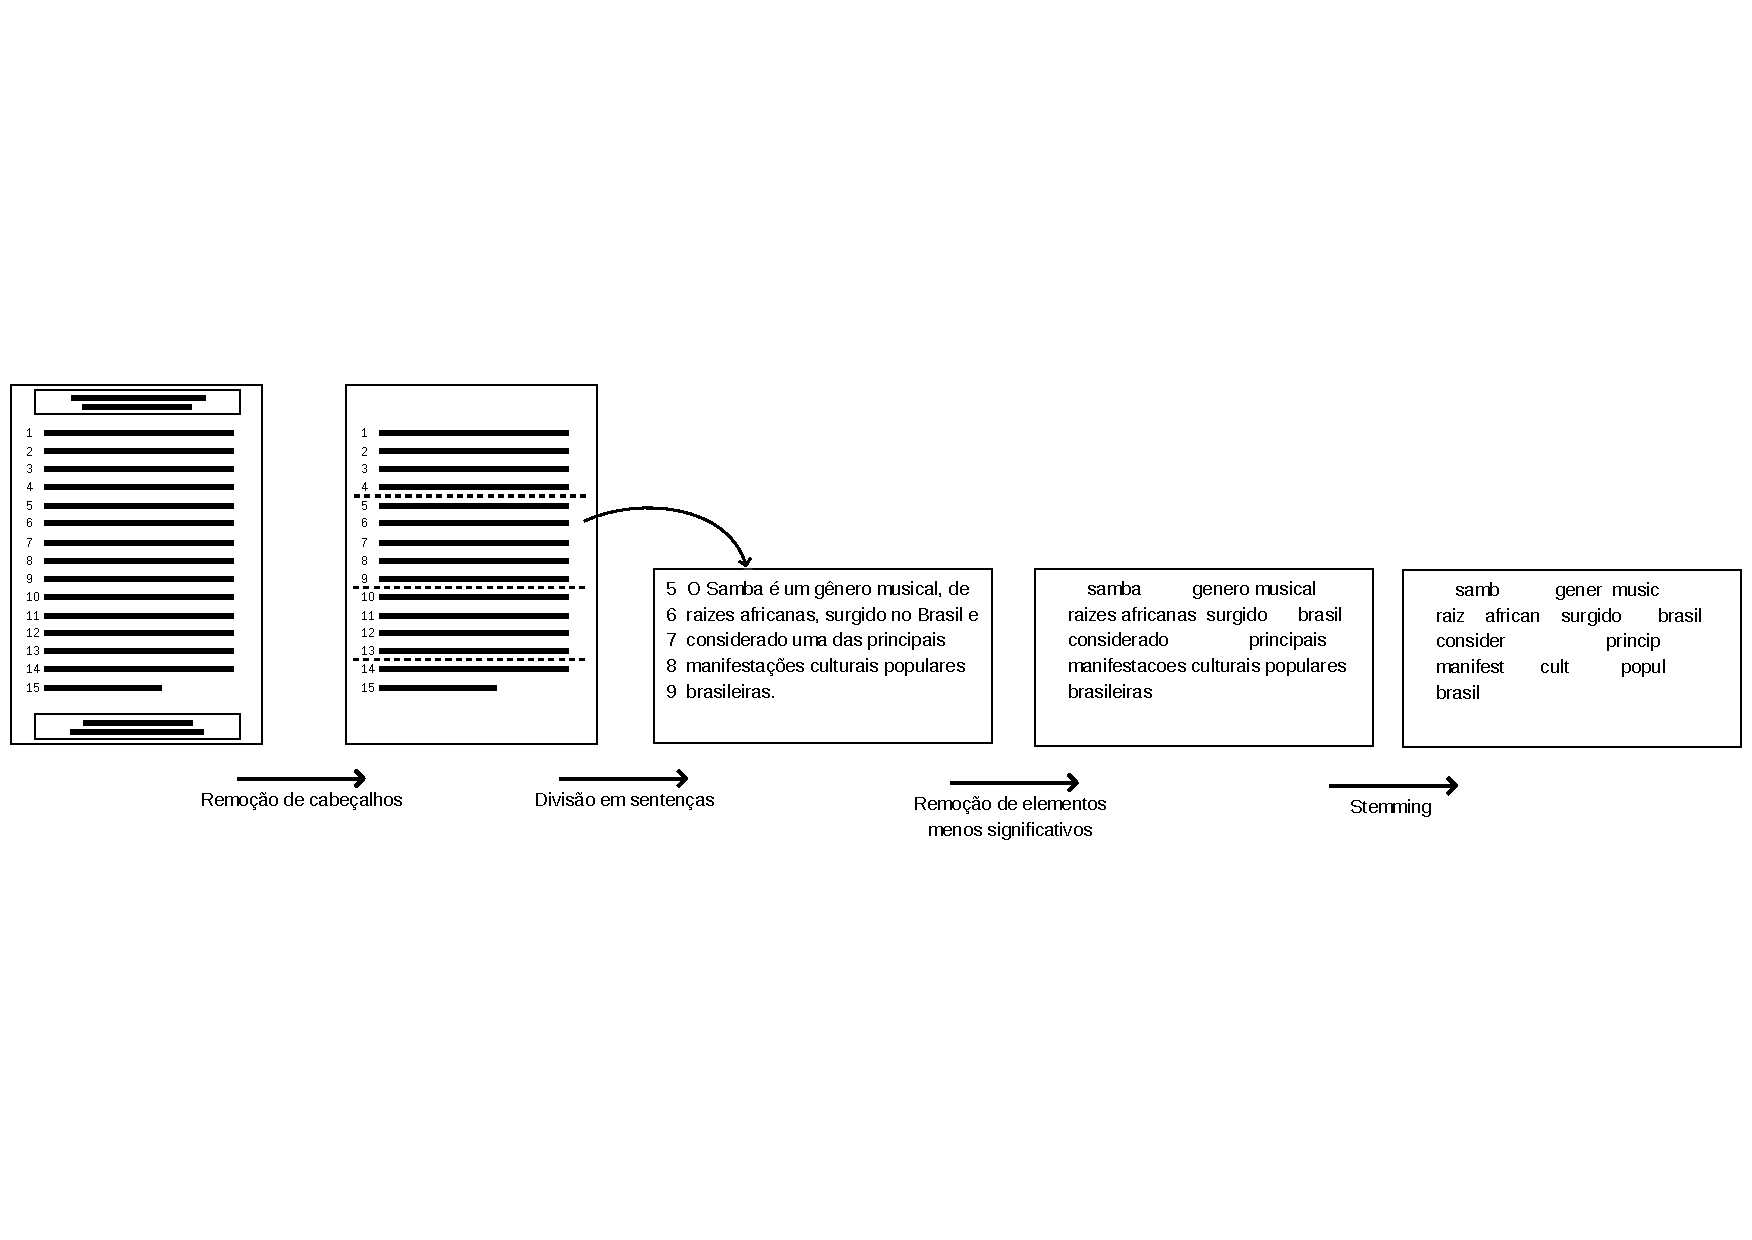
\includegraphics[trim={ 0 180 0 180 },clip,page=1,width=\textwidth]{conteudo/capitulos/figs/pre-process.pdf}

	\caption{Etapa de pré-processamento de um documento que inclui da remoção de elementos menos significativos e a identificação de sentenças}
	\label{fig:preprocessamento-segmentacao}
	\end{figure}
\end{center}



\begin{enumerate}

%  Cabeçalhos e rodapés
\item Remoção de cabeçalhos: as atas contém trechos que podem ser considerados pouco informativos e descartados durante o pré-processamento, como cabeçalhos e rodapés que se misturam aos tópicos tratados na reunião, podendo ser inseridos no meio de um tópico prejudicando tanto os algoritmos de MT e RI, quanto a leitura do texto pelo usuário. Um cabeçalho é a porção de texto que inicia cada página do documento e, de forma semelhante, um rodapé e a porção que as encerra. Detecta-se os cabeçalhos e os rodapés sempre que há uma repetição das primeiras e últimas palavras do documento.


%  Identificação de sentenças
\item Identificação sentenças: Nesse trabalho considera-se as sentenças as menor unidade de informação a ser processada pelos algoritmos de segmentação, por tanto, devem ser identificadas. Ao considerar intuitivamente que uma sentença seja uma sequência de palavras entre sinais de pontuação como ``.'', ``!'' e ``?'', alguns erros poderiam ocorrer quando esses tiverem outra função dentro do texto como em abreviações\footnote{As abreviações são identificadas por meio de uma lista com 234 abreviações conhecidas.}, endereços de internet e datas. Outro problema seriam frases curtas com poucas palavras e que não expressam um conceito completo, mas parte dele. Devido ao estilo de pontuação desses documentos, como encerrar sentenças usando um \textit{``;''} e inserção de linhas extras, foram usadas as regras especiais para identificação de finais de sentença. No Algoritmo~\ref{alg:identificacaofinaisdesent} é mostrado como cada \textit{token} é identificado e marcado com final de sentença.%, esse processo é melhor descrito na Subseção~\ref{subsec:indentificacaosentencas}. % Os detalhes sobre essas regras estão disponíveis para consulta em \urlsoftwares.



\begin{algorithm}
	\SetKwInOut{Input}{Entrada}
	\SetKwInOut{Output}{Saída}
	\SetKwBlock{Inicio}{início}{fim}
	\SetKwFor{ParaTodo}{para todo}{}{fim para todo}
	\SetKwIF{Se}{SenaoSe}{Senao}{}{}{senao se}{senao}{fim se}
	\SetKwFor{Para}{}{}{}
%	\SetKwAlgorithm{Algorithm}{Algoritmo}{}

	
	\Input{Texto}
	\Output{Texto com identificações de finais de sentença}
	
	\ParaTodo {token, marcá-lo como final de sentença se:} {	

	Terminar com um \texttt{!}\\
	Terminar com um \texttt{.} e não for uma abreviação\\
	Terminar em \texttt{.?;} e:
		\Para{}{
			For seguido de uma quebra de parágrafo ou tabulação\\
			O próximo \textit{token} iniciar com  \texttt{(\{["'}\\
			O próximo \textit{token} iniciar com letra maiúscula\\
			O penúltimo caracter  for \texttt{)\}]"'}\\
		}
	}
	
	\caption{Identificação de finais de sentença.}
	\label{alg:identificacaofinaisdesent}
\end{algorithm}


% TODO: "Pra que fazer isso?"


%  Remoção de termos
\item Redução de elementos menos significativos: Removeu-se do textos os termos que não contribuem para a etapa de segmentação, 
	as quais são chamadas de \textit{stop words}. Palavras como artigos, preposições, pronomes, verbos de estado\footnote{Apresentam uma situação inativa, onde o verbo não expressa uma alteração, mas apenas uma propriedade ou condição dos envolvidos.}. Trata-se também como \textit{stop words} as palavras de uso muito frequente dentro de um determinado domínio as quais não são capazes de discriminar textos, portanto também não devem fazer parte dos atributos~\cite{Rezende2003}. Para removê-las, as letras foram convertidas em caixa baixa e usou-se uma lista de 438 palavras para identificá-las. Além disso, eliminou-se a acentuação, sinais de pontuação, numerais e todos os termos menores que três caracteres.

%  Stemming
\item \textit{Stemming}: extraiu-se o radical de cada palavra. Para isso, aplicou-se o algoritmo \textit{Orengo} %\footnote{http://www.inf.ufrgs.br/~viviane/rslp/} 
	para remoção de sufixos~\cite{Alvares2005}.

\end{enumerate}
	


% ---------------------------------------------------------------------------------
% ---------------------------------------------------------------------------------




















































Ao final gerou-se para cada documento uma texto 



"A profª AAA informou que hoje dia cinco de agosto às 14 horas acontecerá a reunião de estruturação do campus e a profª BBB aproveita para esclarecer que essas reuniões tem como objetivo fechar as propostas para que sejam enviadas juntamente com as propostas dos departamentos.",informe,,reunião;estruturação;campus;
"A respeito do PPP do curso da Ciência da Computação a profª AAA informou que o mesmo já está em fase de avaliação na ProGrad e que a comissão que irá avaliá-lo já foi definida.",informe,,ppp;ciência;computação;
"Comunicação dos Membros: O prof. CCC informou que o prof. DDD desistiu de pedir transferência para o nosso campus.",informe,,transferência;desistiu;



\begin{table}[!h]
	\centering 
\footnotesize
	\begin{tabular}{|p{0.2cm}p{14,5cm}|} \hline

		$^{[11]}$&A profª AAA informou que hoje dia cinco de agosto às 14 horas acontecerá a reunião de estruturação do campus e a profª BBB aproveita para esclarecer que essas reuniões tem como objetivo fechar as propostas para que sejam enviadas juntamente com as propostas dos departamentos.
 \\

		$^{[12]}$ &
		A respeito do PPP do curso da Ciência da Computação a profª AAA informou que o mesmo já está em fase de avaliação na ProGrad e que a comissão que irá avaliá-lo já foi definida.\\

		$^{[13]}$ &
		Comunicação dos Membros: O prof. CCC informou que o prof. DDD desistiu de pedir transferência para o nosso campus. 

	\end{tabular}
	\caption{Exemplo de }
	\label{tab:segmentacaoreferencia}
\end{table}










"(II) Encerrada a etapa de inscrição para o processo seletivo como aluno regular para o segundo semestre de 2015: foram quarenta e nove inscrições on-line e dezoito candidatos entregaram a documentação;",informe,,processo;seletivo;

"(III) O Prof. Dr. Alexandre Alvaro informou que a Pró- Reitora comunicou a oferta de mais uma bolsa pela cota da Pró-Reitoria, mas não havia aluno disponível para alocação da bolsa.
O Prof. Dr. José de Oliveira Guimarães informou que havia uma aluna interessada, mas não informada durante o processo de elaboração do ranking no início do semestre.
Ficou decidido enviar e-mail aos docentes solicitando que comuniquem permanentemente interesse de alunos em bolsa pra atualização do ranking;",informe,solicitação;,bolsa;cota;ranking;alunos;
"(IV) Com a mudança do Prof. Dr. Murillo Rodrigo Petrucelli Homem para o campus de São Carlos, o Prof. Dr. José de Oliveira Guimarães assume o posto de suplente da linha Teoria Aplicada à Computação na CPG;",informe,,mudança;suplente;teoria;aplicada;computação;
"Comunicação dos membros: Não houve;",irrelevante,,
"Ordem do Dia: (I) Foram apresentadas regras para participação de membro externo em banca de defesa do mestrado.
O Prof. Dr. Alexandre Alvaro comentou que está sendo pago aos participantes externos das bancas a diária pelo PROAP e o pró-labore pelo DComp, além do programa fornecer o transporte, que onera a verba PROAP.
O Prof. Dr. Tiago Agostinho de Almeida sugeriu o seguinte cálculo para pagamento: se o participante vier de uma Instituição com distância até 220 km será feito o cálculo de R$ 1,00 multiplicado pela quilometragem.
Caso a distância seja superior a 220 km, será calculada a distância multiplicada por R$ 0,60. O menor valor entre o custo do transporte e o pagamento de verba e pró-labore será utilizado para custear a vinda do participante;",informe,discussão;,banca;participantes;diária;transporte;custo;
"(II) Foi discutida a forma de convalidação de disciplinas cursadas como aluno regular anterior a três anos do reingresso do aluno.
Foi decidido que fica a cargo da CPG decidir sobre as disciplinas que serão aproveitadas quando do reingresso do aluno;",decisão,discussão;,disciplinas;aluno;regular;convalidação;

































01 Ata 30 - 26a Reunião Odinária PPGCCS.txt.csv
 7 & 4 & 11 & 6 & 16 & 8 & 8 & 15 & 16 & 
	Anotador  1   7 segmetnos |  25 sentenças
	Anotador  2   4 segmetnos |  25 sentenças
	Anotador  3  11 segmetnos |  25 sentenças
	Anotador  4   6 segmetnos |  25 sentenças
	Anotador  5  16 segmetnos |  25 sentenças
	Anotador  6   8 segmetnos |  25 sentenças
	Anotador  7   8 segmetnos |  25 sentenças
	Anotador  8  15 segmetnos |  25 sentenças
	Anotador  9  16 segmetnos |  25 sentenças
02 Ata 29 - 25a Reunião Odinária PPGCCS.txt.csv
 4 & 4 & 8 & 6 & 11 & 6 & 6 & 15 & 14 & 
	Anotador  1   4 segmetnos |  17 sentenças
	Anotador  2   4 segmetnos |  17 sentenças
	Anotador  3   8 segmetnos |  17 sentenças
	Anotador  4   6 segmetnos |  17 sentenças
	Anotador  5  11 segmetnos |  17 sentenças
	Anotador  6   6 segmetnos |  17 sentenças
	Anotador  7   6 segmetnos |  17 sentenças
	Anotador  8  15 segmetnos |  17 sentenças
	Anotador  9  14 segmetnos |  17 sentenças
03 Ata 36 - 31a Reunião Odinária PPGCCS.txt.csv


 6  & 6  & 8  & 4  & 15 & 9  & 10 & 18 & 14 & 

	Anotador  1   6 segmetnos |  26 sentenças
	Anotador  2   6 segmetnos |  26 sentenças
	Anotador  3   8 segmetnos |  26 sentenças
	Anotador  4   4 segmetnos |  26 sentenças
	Anotador  5  15 segmetnos |  26 sentenças
	Anotador  6   9 segmetnos |  26 sentenças
	Anotador  7  10 segmetnos |  26 sentenças
	Anotador  8  18 segmetnos |  26 sentenças
	Anotador  9  14 segmetnos |  26 sentenças
04 Ata 32 - 28a Reunião Odinária PPGCCS.txt.csv


 5 & 5 & 10 & 6 & 14 & 17 & 7 & 11 & 12 &

	Anotador  1   5 segmetnos |  26 sentenças
	Anotador  2   5 segmetnos |  26 sentenças
	Anotador  3  10 segmetnos |  26 sentenças
	Anotador  4   6 segmetnos |  26 sentenças
	Anotador  5  14 segmetnos |  26 sentenças
	Anotador  6  17 segmetnos |  26 sentenças
	Anotador  7   7 segmetnos |  26 sentenças
	Anotador  8  11 segmetnos |  26 sentenças
	Anotador  9  12 segmetnos |  26 sentenças
05 Ata 33 - 29a Reunião Odinária PPGCCS.txt.csv

 4 & 4 & 6 & 5 & 17 & 22 & 9 & 18 & 16 &

	Anotador  1   4 segmetnos |  33 sentenças
	Anotador  2   4 segmetnos |  33 sentenças
	Anotador  3   6 segmetnos |  33 sentenças
	Anotador  4   5 segmetnos |  33 sentenças
	Anotador  5  17 segmetnos |  33 sentenças
	Anotador  6  22 segmetnos |  33 sentenças
	Anotador  7   9 segmetnos |  33 sentenças
	Anotador  8  18 segmetnos |  33 sentenças
	Anotador  9  16 segmetnos |  33 sentenças
06 Ata 35 - 5a Reunião Extraodinária PPGCCS.txt.csv

3 & 4 & 6 & 4 & 9 & 9 & 4 & 7 & 5 &




	Anotador  1   3 segmetnos |  11 sentenças
	Anotador  2   4 segmetnos |  11 sentenças
	Anotador  3   6 segmetnos |  11 sentenças
	Anotador  4   4 segmetnos |  11 sentenças
	Anotador  5   9 segmetnos |  11 sentenças
	Anotador  6   9 segmetnos |  11 sentenças
	Anotador  7   4 segmetnos |  11 sentenças
	Anotador  8   7 segmetnos |  11 sentenças
	Anotador  9   5 segmetnos |  11 sentenças
07 20ª Reunião Extraordinária CoC-CCS 08-12-10.txt.csv

 3 & 7 & 5 & 4 & 11 & 14 & 5 & 5 & 4 &




	Anotador  1   3 segmetnos |  20 sentenças
	Anotador  2   7 segmetnos |  20 sentenças
	Anotador  3   5 segmetnos |  20 sentenças
	Anotador  4   4 segmetnos |  20 sentenças
	Anotador  5  11 segmetnos |  20 sentenças
	Anotador  6  14 segmetnos |  20 sentenças
	Anotador  7   5 segmetnos |  20 sentenças
	Anotador  8   5 segmetnos |  20 sentenças
	Anotador  9   4 segmetnos |  20 sentenças
08 25ª Reunião Ordinária CoC-CCS 04-04-12.txt.csv

 4 & 8 & 3 & 8 & 12 & 17 & 5 & 11 & 9 &


	Anotador  1   4 segmetnos |  35 sentenças
	Anotador  2   8 segmetnos |  35 sentenças
	Anotador  3   3 segmetnos |  35 sentenças
	Anotador  4   8 segmetnos |  35 sentenças
	Anotador  5  12 segmetnos |  35 sentenças
	Anotador  6  17 segmetnos |  35 sentenças
	Anotador  7   5 segmetnos |  35 sentenças
	Anotador  8  11 segmetnos |  35 sentenças
	Anotador  9   9 segmetnos |  35 sentenças
09 40ª Reunião Ordinária CoC-CCS 06-05-15.txt.csv

3 & 5 & 3 & 6 & 11 & 11 & 3 & 9 & 9 &

	Anotador  1   3 segmetnos |  24 sentenças
	Anotador  2   5 segmetnos |  24 sentenças
	Anotador  3   3 segmetnos |  24 sentenças
	Anotador  4   6 segmetnos |  24 sentenças
	Anotador  5  11 segmetnos |  24 sentenças
	Anotador  6  11 segmetnos |  24 sentenças
	Anotador  7   3 segmetnos |  24 sentenças
	Anotador  8   9 segmetnos |  24 sentenças
	Anotador  9   9 segmetnos |  24 sentenças
10 20ª Reunião Ordinária CoC-CCS 01-06-11.txt.csv

 4 & 5 & 4 & 7 & 31 & 29 & 5 & 9 & 8 &

	Anotador  1   4 segmetnos |  50 sentenças
	Anotador  2   5 segmetnos |  50 sentenças
	Anotador  3   4 segmetnos |  50 sentenças
	Anotador  4   7 segmetnos |  50 sentenças
	Anotador  5  31 segmetnos |  50 sentenças
	Anotador  6  29 segmetnos |  50 sentenças
	Anotador  7   5 segmetnos |  50 sentenças
	Anotador  8   9 segmetnos |  50 sentenças
	Anotador  9   8 segmetnos |  50 sentenças
11 10ª Reunião Ordinária CoC-CCS 05-04-10.txt.csv


4 & 7 & 5 & 7 & 29 & 19 & 5 & 9 & 12 &


	Anotador  1   4 segmetnos |  43 sentenças
	Anotador  2   7 segmetnos |  43 sentenças
	Anotador  3   5 segmetnos |  43 sentenças
	Anotador  4   7 segmetnos |  43 sentenças
	Anotador  5  29 segmetnos |  43 sentenças
	Anotador  6  19 segmetnos |  43 sentenças
	Anotador  7   5 segmetnos |  43 sentenças
	Anotador  8   9 segmetnos |  43 sentenças
	Anotador  9  12 segmetnos |  43 sentenças
12 13ª Reunião Ordinária CoC-CCS 05-08-10.txt.csv

3 & 10 & 4 & 16 & 33 & 25 & 4 & 13 & 11 &


	Anotador  1   3 segmetnos |  56 sentenças
	Anotador  2  10 segmetnos |  56 sentenças
	Anotador  3   4 segmetnos |  56 sentenças
	Anotador  4  16 segmetnos |  56 sentenças
	Anotador  5  33 segmetnos |  56 sentenças
	Anotador  6  25 segmetnos |  56 sentenças
	Anotador  7   4 segmetnos |  56 sentenças
	Anotador  8  13 segmetnos |  56 sentenças
	Anotador  9  11 segmetnos |  56 sentenças




% Entre os principais trabalhos da literatura podemos citar o \textit{TextTiling} ~\cite{Hearst1994} e o \textit{C99}~\cite{Choi2000} são considerados um dos primeiros mais influentes sendo utilizados com \textiit{base lines} em trabalhos recentes~\cite{CHAIBI2014, Naili2016, Cardoso2017}


% para então ser segmentação do texto em trechos com um assunto predominante. 
% conforme apresentados a seguir.

% melhorar ↓↓↓↓↓
% A seguir são apresentadas as etapas do módulo de preparação e manutenção desde a preparação dos documentos até a entrega da estrutura interna ao módulo de consulta. 





% A Figura~\ref{fig:preprocessamento-segmentacao} mostra a etapa de preparação de um documento em português que inclui a remoção de elementos menos significativos e a identificação de sentenças e segmentos.


  % A Figura \ref{fig:visao-geral} mostra a visão geral do sistema com suas principais entradas e saídas. 



e devolve o histórico de menções 


informações extraídas


0. Extração e preparação do texto

1. Segmentação dos documentos

2. Extração dos tópicos


















% --> Encerramento da seção de segmentação.
Ao final do processo de segmentação, são produzidos fragmentos de documentos, aqui chamados de subdocumentos. Esses subdocumentos contém um texto, assim como no documento original, em um estágio de processamento inicial, pois ainda não estão estruturados. Ocorre que as técnicas de aprendizado de máquina exigem uma representação estruturada dos textos conforme será visto na Seção~\ref{section:RepTextos}.




% Analisou-se também o desempenho da mesma técnica aplicada a um texto contínuo extraído de artigo da Internet que descreve seis gêneros musicais brasileiros um após um outro separados em seções. Ao observar a Figura~\ref{fig:coesaolexicaTT-generos-musicais}, nota-se que os vales são mais definidos e a maioria dos segmentos coincidem ou estão próximos a segmentação de referência. A segmentação de referência possui sete segmentos que separam uma introdução do assuntos e respeitam cada uma das subseções que tratam de um gênero musical. Obtém-se nesse cenário uma eficiência maior em relação a segmentação da ata, o que sugere que textos organizados em seções podem ter melhores benefícios com técnicas baseadas em coesão léxica que as atas, onde esse fator é menos significativo.  % ou a premissa do algoritmo não é tão boa.



  % %--- ---
  % \begin{figure}[!h]
	  % \centering
	  % 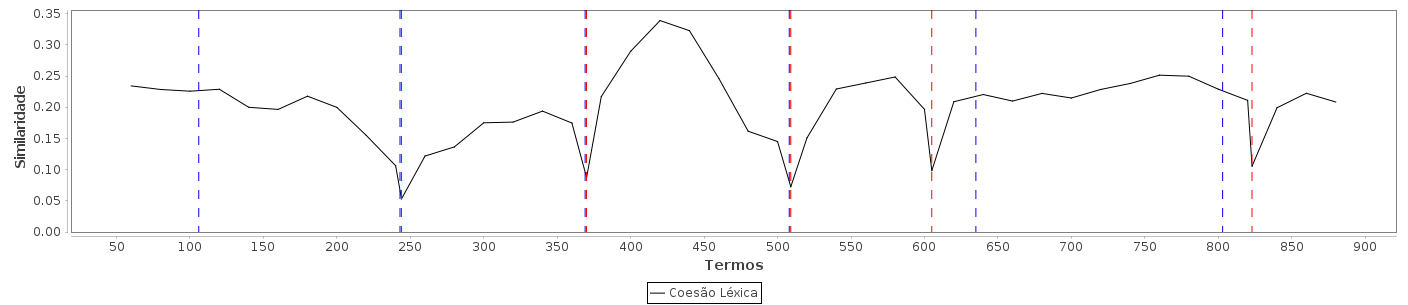
\includegraphics[width=\textwidth]{conteudo/capitulos/figs/generos-musicais-TT-40-20.png}
	  % \caption{Variação da coesão léxica ao longo de um artigo melhor estruturado em seções junto a uma segmentação automática em contraste com uma segmentação de referência.}
	  % \label{fig:coesaolexicaTT-generos-musicais}
  % \end{figure}




% O usuário final precisa de uma interface adequada para visualizar os resultados retornados pela busca considerando-se a relevância dos segmentos selecionados e a navegação pelos tópicos. Uma boa apresentação deve permitir ao usuário identificar a os resultados e ser relativante suficiente para compreensão do conteúdo, evitando a leitura do texto completo. Ou seja, o texto de cada segmento apresentado deve ser suficiente para compreensão do assunto mencionado, sem necessidade de visualizar o documento original.




% O módulo de preparação e manutenção tem como função principal manter uma base de dados necessária para os processos de recuperação de informação. Primeiramente, esse módulo deve receber um conjunto inicial de documentos os quais devem ser divididos em segmentos de texto que contêm um assunto predominante, e agrupá-los em categorias por meio de técnicas de extração de tópicos. Além disso, considera-se o crescimento da bases de documentos, assim, o sistema deve receber novos documentos a medida que são gerados. 




% Esse capítulo está organizado da seguinte forma: primeiramente, na Seção~\ref{sec:sistema-proposto} é apresentada uma visão geral do sistema proposto, seu funcionamento e como as técnicas de segmentação textual e extração de tópicos são empregadas para gerar uma base de dados que concentra as informações necessárias para identificar e agrupar os diversos assuntos distribuídos na coleção de documentos. Ainda nessa seção, são apresentadas as técnicas de recuperação de informação utilizadas para entregar os segmentos de acordo com a consulta do usuário bem como permitir a exploração de segmentos relacionados ao mesmo tema, os quais originalmente estão distribuídos na coleção de documentos.  



% Na Seção~\ref{sec:aplicacao-sistema} é apresentada a aplicação do sistema proposto ao contexto das atas de reunião, ou seja, utilizando como base de dados uma coleção de atas de reunião. Uma vez que as atas configuram um corpus com documentos multi-temáticos, conforme a proposta desse trabalho, essa aplicação visa a validação do sistema e a análise da eficiência das técnicas empregadas em um \textit{corpus} em conformidade com a proposta desse trabalho de mestrado. Será apresentada também a preparação das atas, a descrição dos algoritmos utilizados e suas configurações.



% Na etapa de pré-processamento, os documentos são pré-processados individualmente conforme são recebidos pelos algoritmos de segmentação extração de tópicos. Inicialmente, cada texto passou por um processo de transformação em que as letras foram convertidas em caixa baixa e eliminou-se sinais de pontuação, numerais e termos menores que três caracteres. Em seguida removeu-se os termos que não contribuem para a etapa de segmentação, as quais são chamadas de \textit{stop words}, para identificá-las usou-se uma lista de 438 palavras. Em seguida, extraiu-se o radical de cada palavra por meio da técnica \textit{stemming}. 




% Na Figura~\ref{fig:estrutura-dados-interna} é apresentado a visão geral da estrutura de dados interna.  Na Figura~\ref{fig:estrutura-dados-interna} ilustra-se os arquivos da coleção de documentos ($D$) que contêm assuntos diversos (representados pelos círculos, quadrados e triângulos) ficando disponíveis para visualização e fonte original das informações. Os arquivos originais são mantidos para referência aos textos integrais fincando disponíveis para visualização e fonte original das informações. 



% Após a etapa de extração de tópicos utilizada com um conjunto de segmentos adiciona informações a estes e cria uma base de dados derivada do \textit{corpus} original, a qual é descrita na seção a seguir.
